\documentclass{article}
\usepackage[margin=1in]{geometry}
\usepackage{mathtools}
\usepackage{verbatim}

\usepackage{amsthm}
\theoremstyle{definition}
\newtheorem*{lemma}{Lemma}
\newtheorem*{note}{Note}

\usepackage[charter]{mathdesign}
\usepackage{inconsolata}

\usepackage{graphicx}

\let\P=\relax
\DeclareMathOperator{\E}{\mathbf{E}}
\DeclareMathOperator{\P}{\mathbf{P}}

\begin{document}
{\fontfamily{ccr}\selectfont
  \begin{center}
    {\Large AM 225: Homework \#1}\\
Kevin Li \quad 15 February 2019 \\
  \end{center}
}

\section*{Preliminaries}
The code is found in the \texttt{code} folder; all of the code is mine,
except for two external libraries. The first external library (called \texttt{fmt})
is a pretty-format library similar in spirit to Python's format function e.g.,
\begin{verbatim}fmt::print("Hello, {}.\n", "Chris");
\end{verbatim}
instead of more verbose \texttt{std::cout} statements.
The second external library (called \texttt{cleantype})
allows for easy printing of STL containers. Clearly, neither of these
libraries are essential to the logic of the problems.
The code for these two libraries lives in the \texttt{common} folder;
thus, all code in the \texttt{code} directory was written by me.

Inside the \texttt{code} folder, type \texttt{make} to
generate executables. You will need a C++14 compatible compiler;
on my Linux system, I use GCC 7.3.0. The executables
all have a \texttt{.bin} extension, i.e.,
\begin{verbatim}
<name>.bin,      for example: one.bin, two-a.bin, etc.
\end{verbatim}
The source code is named in a self-explanatory way (e.g., \texttt{problem4c.cpp}).
There is a small utility class called \texttt{timer} which prints out
the execution timer in milliseconds.


\section{Problem 1}
\subsection{Part (a)}
According to the simulations, the expected winnings (in dollars)
is $21.8308$ per round. Therefore, the game is worth playing (for a 
risk-neutral agent). The running time (in milliseconds) are
\begin{verbatim}
threads time    profit
1       28786.8 21.8335
2       14410.8 21.8276
4       7203.43 21.826
\end{verbatim}
This is good: we have roughly linearly scaling with the number of threads.
(The third column is redundant.)

\subsection{Part (b)}
The following lemma is easily proven by induction. 
\begin{lemma}
Let $U_1, \dots, U_n$ be independent random variables uniformly distributed
on the unit interval $[0, 1]$. For any $t \in [0, 1]$
\begin{equation}
\P(U_1 + \dots + U_n \leq t) = \frac{t^n}{n!}.
\end{equation}
\end{lemma}

We draw strictly more than $n$ numbers
in the lottery game if and only if $U_1 + \dots + U_n \leq 1$. This occurs
with probability $1/n!$, so that the expected number of draws\footnote{Recall that
for a non-negative integer-valued random variable $X$,
\begin{equation*}
  \E X = \P(X > 0) + \P(X > 1) + \P(X > 2) + \dots.
\end{equation*}} is
\begin{equation}
\sum_{k=0}^{\infty} \frac{1}{n!} = e.
\end{equation}
The expected winnings therefore $100 e - 250$ dollars. This matches with our
answer in \textbf{Part (a)}.

\section{Problem 2}
\begin{note}
See the files \texttt{grid.h} and \texttt{grid.cpp} for this problem.
The files \texttt{problem2{a,b}} just calls the code in the grid class.
\end{note}

\subsection{Part (a)}
Run the \texttt{two-a.bin} executable to see a print out
of the grid. For convenience, I piped that to the file
\texttt{problem2a.txt}.

\subsection{Part (b)}
The raw data could be generated by running \texttt{two-b.bin}.
I calculate $p(n,T)$ manually in Excel, and the result is saved
in \texttt{problem2.csv}. The attached \texttt{R} code generates the graphics
in \textbf{Part (c)}.


\subsection{Part (c)}
See Figure~\ref{2c} on page~\pageref{2c}. We see two patterns
\begin{enumerate}
\item For fixed $n$, increasing the number of threads generally
decreases thread efficiency. This makes sense: since I lay out my grid
in a one dimensional array, there is some degree of false sharing,
where multiple threads need to access the same cache line at the same time.
There is of course also a penalty for starting threads in the first place.

\item For fixed $T$ (number of threads), thread efficiency increases
as $n$ grows. This also makes sense: there is more parallelism to exploit
in larger problems (the fixed cost of spawning a thread becomes less significant).
To some degree, the false sharing effect is also alleviated in larger grids
(i.e., fewer percentage of accesses exhibit false sharing).

\end{enumerate}
\begin{figure}
  \centering
  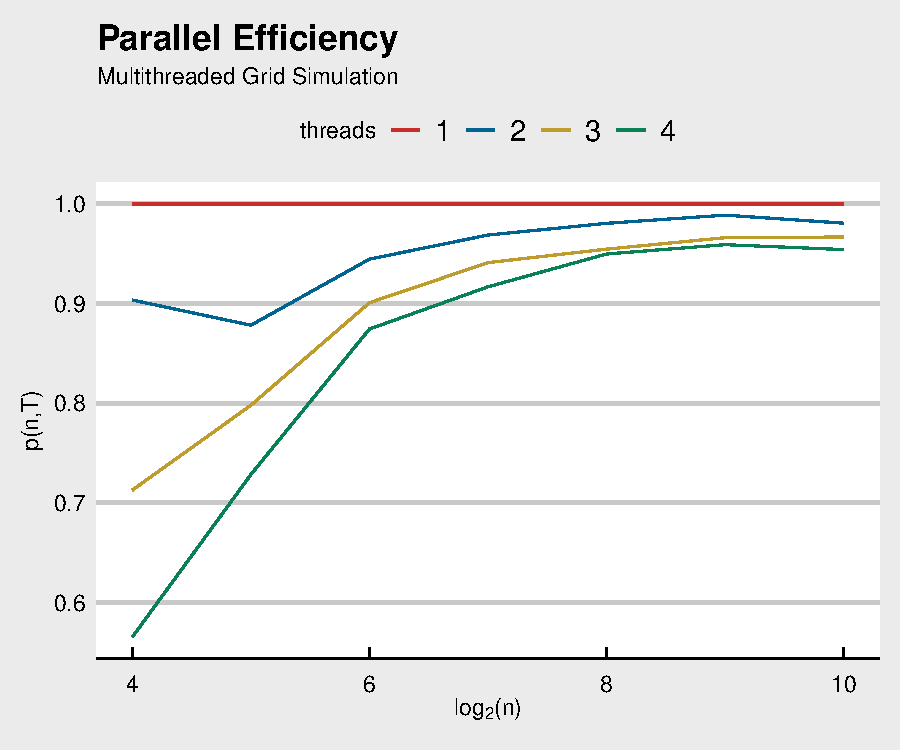
\includegraphics{p2}
\caption{Problem 2c--Parallel efficiency.}
\label{2c}
\end{figure}

\section{Problem 3}
\begin{note}
The code in \texttt{problem3.cpp} and \texttt{problem3.h}
include the helper functions. The code for the parts are in
\texttt{problem3a.cpp}, \texttt{problem3b.cpp}, and so on.
\end{note}

\subsection{Part (a)}
See the text file \texttt{primes.txt} for the list of primes;
there are 17984 of them.


\subsection{Part (b)}
The long division code is in \texttt{problem3.cpp}, under the function
\texttt{long\_division}. The file \texttt{problem3b.cpp}
does a small example that I checked in Mathematica. 

\subsection{Part (c)}
In the base $B = 2^b$, the number $2^n - 1$ may be represented
as
\begin{equation}
2^n - 1 = (2^r-1) (B^q) + (B-1) B^{q-1} + (B-1) B^{q-2} + \dots + (B-1) B + (B-1)
\end{equation}
where $0 \leq r < B$ and $q \geq 0$ are the unique integers satisfying
\begin{equation}
n = bq + r.
\end{equation}
My long division algorithm uses \texttt{uint64} as the underlying integer representation
and the algorithm itself requires that $B^2-1$ fits inside the presentation. Therefore,
I chose $B = 2^{32}$, i.e., $b = 32$.

As expected, there are no prime factors of the Mersenne prime
$2^{82589933} - 1$. (The problem \texttt{three-c.bin} prints every prime
factor, and its produces nothing.)

\subsection{Part (d)}
My program finds prime factors $3$, $5$, and $41201$ as the prime factors
of $N$ below one million. This does take a long time to run, because my
long division code is inefficient. (On my fairly quick six-core desktop,
I waited about 9 minutes.)


\section{Problem 4}
\begin{note}
I made some minor changes to Algorithm 1 to make it more efficient.
The issue is that the given algorithm is too slow to finish
in Part (d) in a reasonable amount of time.

The exact modification is that each the board is actually \emph{copied}
in every recursive call, thus there is no need to remove the guess $j$; the
sudoku board simply goes out of scope. Moreover, every time a new guess is entered,
there is some bookkeeping in the background to make sure that board is
as reduced as possible. Specifically, this means: if a newly entered guess
in square $j$ forces the cell $k$ to admit only one legal value, then the cell $k$
is filled in. If this causes another cell $\ell$ to admit only one legal value,
then $\ell$ is filled in as well, and so on.

The code is found in \texttt{sudoku.cpp} and \texttt{sudoku.h}. Note that
\texttt{ChronoCube} is my GitHub handle, hence the namespace name.

\end{note}

\subsection{Part (a)}
According to the timing produced by \texttt{four-a.bin}, solving the puzzle once
takes approximately $0.07$ milliseconds. Pretty quick!

\subsection{Part (b)}
There are 283576 solutions, as verified.
(Run the problem \texttt{four-b.bin}.)

\subsection{Part (c)}
I timed \textbf{Part (d)} instead of \textbf{Part (c)}, since \textbf{Part (c)} finishes
so quickly (one tenth of a second)
that launching parallel threads overwhelms actual computation.

The parallel algorithm
only parallelizes in the top level of the tree.  I tried to use OpenMP tasks\footnote{Using the task construct of OpenMP seems to be required here because the function we are parallelizing
is recursive.} to parallelize the entire tree; it turns out that simply parallelizing
the top part of the tree yields better performance. 

The timings are 10 seconds; 5.9 seconds; and 3.9 seconds for 1, 2, and 4 threads
(respectively). (The speed gains are not very impressive.)

\begin{note}
The second argument to \texttt{count\_solutions\_parallel} controls the number
of threads. Simply change the call in \textbf{problem4c.cpp} and recompile
and use the shell builtin to time.
\end{note}


\subsection{Part (d)}
There are 4347232 solutions to the puzzle,
as per the verification in \textbf{Part (c)}.

\end{document}
